\documentclass[12pt,a4paper]{article}
\usepackage[utf8]{inputenc}
\usepackage[czech]{babel}
\usepackage[margin=13mm, tmargin=15mm, bmargin=12mm]{geometry}
\usepackage{multirow}
\usepackage{tikz}
\usetikzlibrary{calc}
\usepackage{chngpage}
\usepackage{tabularx}
\usepackage{fancyhdr}
\usepackage{mathptmx}
\usepackage{lipsum}
\usepackage{float}
\usepackage{caption}
\usepackage{subcaption}
\usepackage{pgfplotstable}
\usepackage{booktabs}
\usepackage{siunitx}

\sisetup{
	round-mode = places,
	round-precision = 1,
	separate-uncertainty=true,
	multi-part-units=single,
	output-decimal-marker = {,},
	group-separator = {\ }
}

\renewcommand{\baselinestretch}{1.15}
\pagenumbering{gobble}
\pagestyle{fancy}
\renewcommand{\headrulewidth}{0pt}

\newcommand{\jmeno}{David Škrob, Tomáš Názler, Šimon Skládaný}
\newcommand{\trida}{L4A}
\newcommand{\poradovecislo}{}
\newcommand{\nazevulohy}{Filtry}
\newcommand{\cisloulohy}{}
\newcommand{\predmet}{Technické měření}
\newcommand{\skupina}{}
\newcommand{\datummereni}{2.3.2023}
\newcommand{\datumodevzdani}{3.3.2023}
\newcommand{\klasifikace}{}

\begin{document}
\fancyhead{
\begin{tikzpicture} [overlay,remember picture]
       \draw
        ($ (current page.north west) + (1cm, -12mm) $)
        rectangle
        ($ (current page.south east) + (-1cm,12mm) $);
\end{tikzpicture}
}

\renewcommand{\arraystretch}{2}
\shorthandoff{-}

{
\begin{adjustwidth}[]{-3mm}{-3mm}
\centering
\vspace*{-7mm}
\begin{tabularx}{\linewidth}{l|X|p{3cm}}
\multirow{2}{25mm}{\centering SPŠ a VOŠ technická Brno, Sokolská 1} &
\textbf{LABORATORNÍ CVIČENÍ Z ELEKTROTECHNIKY} & Třída: \trida \\
\cline{2-3}
 & Jméno a příjmení: \jmeno & Poř. Číslo: \poradovecislo \\
\hline
\end{tabularx}

\begin{tabularx}{\linewidth}{X|p{3cm}}
Název úlohy: \nazevulohy & Číslo úlohy: \cisloulohy \\
\hline
Zkoušený předmět: \predmet & Skupina: \skupina \\
\hline
\end{tabularx}

\begin{tabularx}{\linewidth}{X|X|X}
Datum měření: \datummereni &  Datum odevzdání: \datumodevzdani &  Klasifikace: \klasifikace \\
\hline
\end{tabularx}

\end{adjustwidth}
}

\shorthandon{-}

\section*{Teorie}
Pro dolní i horní propust (RC filtr) platí: 
\begin{equation}
	\label{eq}
	f_m = \frac{1}{2\pi R C }
\end{equation}
Kde $f_m$ je mezní frekvence, $R$ je odpor rezistoru a  $C$ je kapacita kondenzátoru.

\section*{Zadání}
Zapojte horní (\ref{fig:HP}) a dolní (\ref{fig:LP}) propust dle schémat.
\begin{figure}[H]
	\centering
	\begin{subfigure}[b]{0.42\textwidth}
		\centering
		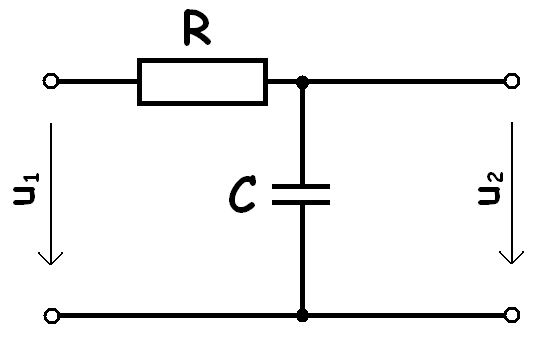
\includegraphics[width=0.85\textwidth]{../../propust/dolniP.png}
		\caption{Dolní propust}
		\label{fig:LP}
	\end{subfigure}
	\hfill
	\begin{subfigure}[b]{0.42\textwidth}
		\centering
		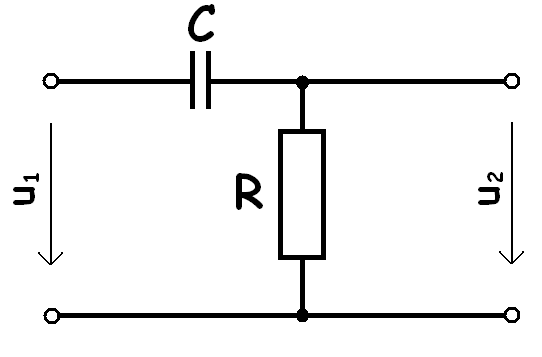
\includegraphics[width=0.85\textwidth]{../../propust/Horni_propust.png}
		\caption{Horní propust}
		\label{fig:HP}
	\end{subfigure}
	\caption{Schémata zapojení}
\end{figure}
Použijte destičky s odpory a kondenzátory. Posílejte sinusový signál z generátoru funkcí a měřte amplitudu na osciloskopu. Změřte $R1$, $R2$, $C1$, $C1$ a vypočítejte mezní frekvenci. Měření proveďte pro frekvence z tabulky
\begin{table}[h!]
	\begin{center}\def\arraystretch{1}
		\caption{Tabulka měřených hodnoty}
		\label{table1}
		\pgfplotstabletypeset[
		1000 sep = {\ },
		dec sep = {,},
		multicolumn names, % allows to have multicolumn names
		col sep=comma, % the seperator in our .csv file
		every head row/.style={
			before row={\hline}, % have a rule at top
			after row={
				\hline} % rule under units
		},
		every last row/.style={after row=\hline}, % rule at bottom
		]{../../propust/freq.csv} % filename/path to file
	\end{center}
\end{table}
\section*{Vypracování}
	R1 = \SI{1}{\kilo\ohm},
	R2 = \SI{5}{\kilo\ohm},
	C1 = \SI{1}{\micro\farad},
	C2 = \SI{0.9}{\micro\farad}.
Tudíž dle vzorce (\ref{eq}) $f_{m1} = \frac{1}{2\pi\cdot \SI{1}{\kilo\ohm}\cdot \SI{1}{\micro\farad}} = \SI{159.15}{\hertz}$ a $f_{m2} = \frac{1}{2\pi\cdot \SI{5}{\kilo\ohm}\cdot \SI{0.9}{\micro\farad}} = \SI{35.36}{\hertz}$
\begin{figure}[H]
	\centering
	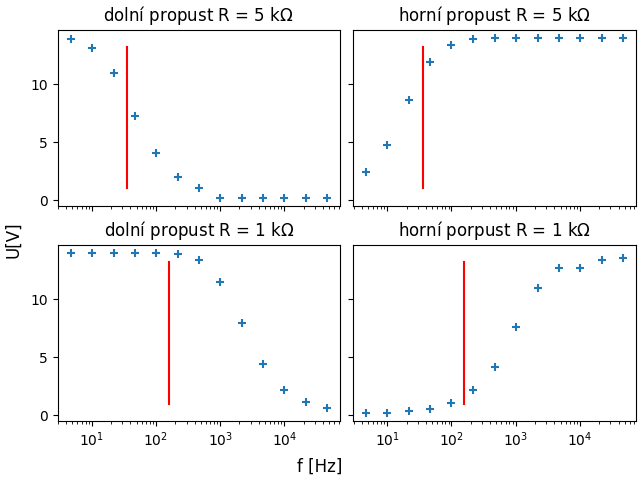
\includegraphics[width=0.9\textwidth]{fancy3.png}
	\caption{Naměřené hodnoty amplitudy, čára ukazuje mezní frekvenci}
\end{figure}
\begin{figure}[H]
	\centering
	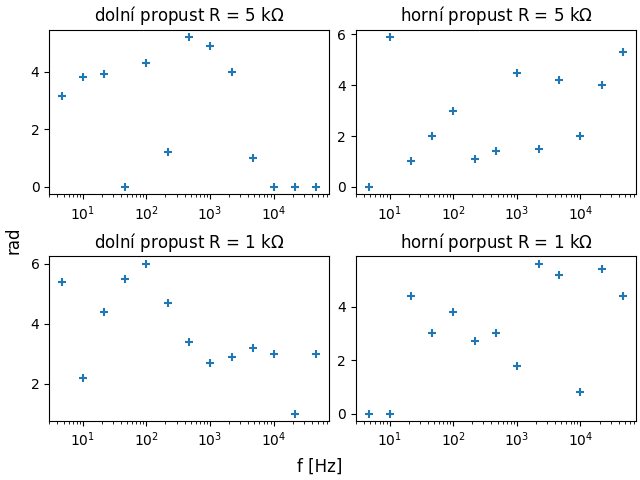
\includegraphics[width=0.9\textwidth]{../../propust/lol1.png}
	\caption{Naměřené hodnoty amplitudy, čára ukazuje mezní frekvenci}
\end{figure}
\section*{Závěr}
Po měření jsme vypočetli mezní frekvenci. Posun fáze vůbec neodpovídá očekávání až na krajní hodnoty, což může být špatným měřením posunu faze osciloskopu. Avšak zeslabení zhruba odpovídá očekávání.
\vfill
\section*{Použité pomůcky:}
\begin{tabularx}{\linewidth}{c|c|c|c}
	Přístroj – pomůcka & Typ & Rozsah (pouze analogové)
	& Poznámka \\
	\hline
	Osciloskop & & &\\
	\hline
	Generátor funkcí & & &Oscilátor\\
\end{tabularx}
\end{document}